\section{Casi d'uso}
\subsection{Introduzione}
In questa sezione vengono descritti i casi d'uso individuati dal gruppo \gruppo{}.
I casi d'uso analizzati fanno riferimento a tutte le funzionalità che il software di sincronizzazione dovrà fornire all'utente finale.\newline
Essendo il progetto finalizzato alla creazione di un applicativo per la sincronizzazione di file, le interazioni da parte dell'utilizzatore sono limitate a pochi e semplici casi d'uso.

\subsection{Attori}

\subsubsection{Attori Principali}
\begin{itemize}
\item \textbf{Utente non autenticato:} È un utente che ha avviato per la prima volta l'applicazione, non è in grado di sincronizzare i file con Zextras Drive fino a quando non effetuerà il login.
\item \textbf{Utente autenticato:} Utente presente nel sistema Zextras, è riconosciuto all'interno dell'applicazione e può usare il programma per sincronizzare i file all'interno di Zextras Drive.
\end{itemize}

\subsubsection{Attori Secondari}
\begin{itemize}
\item \textbf{Gestore credenziali Zextras:} Consente di verificare se le credenziali inserite dall'utente sono presenti all'interno del database di Zextras.
\item \textbf{Zextras Drive:} È un servizio On-premises per conservare i file online, consente di condividere i file presenti nel proprio spazio utente con altri utenti presenti nel sistema. Fornisce delle API con cui è possibile caricare/scaricare file, che sono utili all'applicazione per effettuare la sincronizzazione.
\end{itemize}

\newpage

\subsection{UC1 - Autenticazione}
\begin{figure}[H]
    \centering
    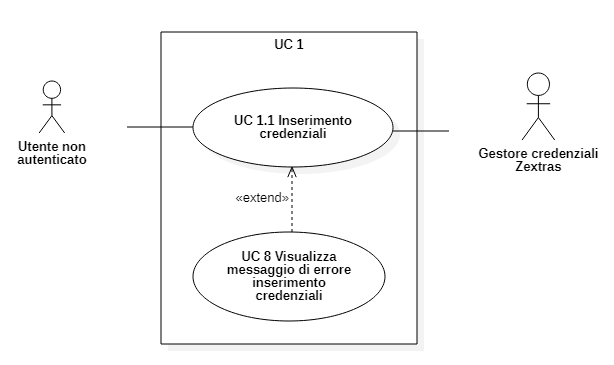
\includegraphics[scale = 0.7]{components/img/UC1.png}
    \caption{UC1 - Autenticazione}
\end{figure}
\subsubsection{UC1.1 - Inserimento credenziali}
\begin{itemize}
\item \textbf{Attore Primario:} Utente;
\item \textbf{Attore Secondario:} Gestore credenziali Zextras;
\item \textbf{Precondizione:} L'utente non è autenticato all'interno dell'applicazione;
\item \textbf{Postcondizione:} L'utente ha effettuato il login usando le credenziali di \glo{Zextras Drive};
\item \textbf{Scenario principale:}
    \begin{enumerate}
    \item L'utente avvia l'applicazione per la prima volta;
    \item L'utente inserisce le credenziali \glo{Zextras Drive};
    \end{enumerate}
\item \textbf{Estensioni:}
\begin{itemize}
\item Visualizzazione messaggio di errore inserimento credenziali (UC1.2 \S{}\ref{UC1.2}).
\end{itemize}
\end{itemize}

\subsubsection{UC1.2 - Visualizzazione messaggio di errore inserimento credenziali}
\label{UC1.2}
\begin{itemize}
\item \textbf{Attore Primario:} Utente non autenticato;
\item \textbf{Precondizione:} Il \glo{sistema} rileva un inserimento di credenziali errate;
\item \textbf{Postcondizione:} L'utente viene informato che le credenziali da lui inserite sono errate;
\item \textbf{Scenario principale:}
    \begin{enumerate}
    \item L'utente ha inserito delle credenziali;
    \item Il \glo{sistema} rileva che le credenziali inserite sono sbagliate.
    \end{enumerate}
\end{itemize}%Autenticazione

\subsection{UC2 - Visualizza impostazioni}
\begin{figure}[H]
    \centering
    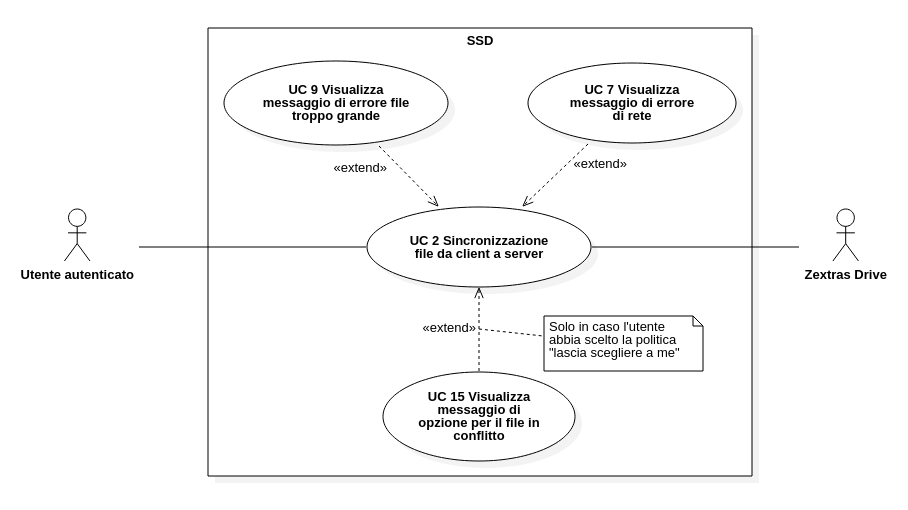
\includegraphics[scale = 0.7]{components/img/UC2.png}
    \caption{UC2 - Visualizza impostazioni}
\end{figure}
\begin{itemize}
\item \textbf{Attore Primario:} Utente autenticato;
\item \textbf{Precondizione:} L'utente vuole visualizzare le impostazioni dell'applicazione;
\item \textbf{Postcondizione:} L'utente può scegliere che impostazioni modificare;
\item \textbf{Scenario principale:}
    \begin{enumerate}
    \item L'utente entra nelle impostazioni;
    \item L'utente può vedere cosa può cambiare all'interno dell'applicazione.
    \end{enumerate}
\end{itemize}

\subsubsection{UC2.1 - Seleziona file da sincronizzare dal client al server}
\begin{figure}[H]
    \centering
    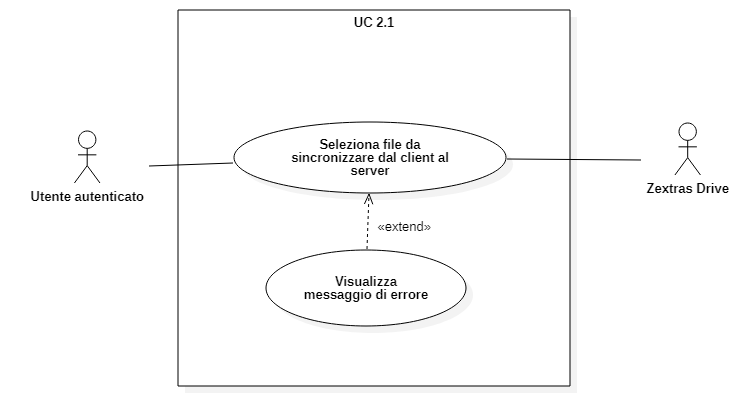
\includegraphics[scale = 0.6]{components/img/UC2_1.png}
    \caption{UC2.1 - Seleziona file da sincronizzare dal client al server}
\end{figure}
\begin{itemize}
\item \textbf{Attore Primario:} Utente autenticato;
\item \textbf{Attore Secondario:} \glo{Zextras Drive};
\item \textbf{Precondizione:} L'utente non ha selezionato nessun file da sincronizzare con il server;
\item \textbf{Postcondizione:} L'utente ha aggiunto dei file che verranno sincronizzati con il server;
\item \textbf{Scenario principale:}
    \begin{enumerate}
    \item L'utente sceglie di aggiungere dei file da sincronizzare con il server;
    \item L'utente aggiunge i file che vuole sincronizzare ad una lista presente nell'applicazione.
    \end{enumerate}
\item \textbf{Estensioni:}
    \begin{itemize}
    \item Visualizzazione messaggio di errore di rete (UC5 \S{}\ref{UC5});
    \item Visualizzazione messaggio di errore file troppo grande (UC6 \S{}\ref{UC6});
    \end{itemize}
\end{itemize}

\subsubsection{UC2.2 - Seleziona file da sincronizzare dal server al client}
\begin{figure}[H]
    \centering
    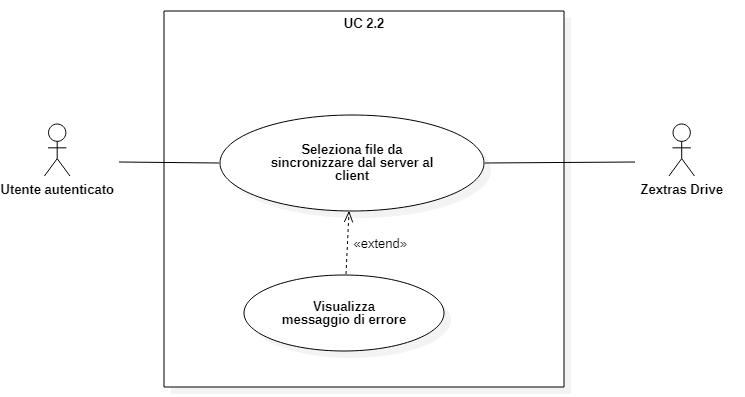
\includegraphics[scale = 0.6]{components/img/UC2_2.png}
    \caption{UC2.2 - Seleziona file da sincronizzare dal server al client}
\end{figure}
\begin{itemize}
\item \textbf{Attore Primario:} Utente autenticato;
\item \textbf{Attore Secondario:} \glo{Zextras Drive};
\item \textbf{Precondizione:} L'utente non ha selezionato nessun file da sincronizzare con il client;
\item \textbf{Postcondizione:} L'utente ha aggiunto dei file che verranno sincronizzati con il client;
\item \textbf{Scenario principale:}
    \begin{enumerate}
    \item L'utente sceglie di aggiungere dei file da sincronizzare con il client;
    \item L'utente aggiunge i file che vuole sincronizzare con il client da una lista presente nell'applicazione.
    \end{enumerate}
\item \textbf{Estensioni:}
    \begin{itemize}
    \item Visualizzazione messaggio di errore di rete (UC5 \S{}\ref{UC5});
    \item Visualizzazione messaggio di errore spazio non disponibile in locale (UC7 \S{}\ref{UC7});
    \end{itemize}
\end{itemize}

\subsubsection{UC2.3 - Seleziona quota disco}
\begin{figure}[H]
    \centering
    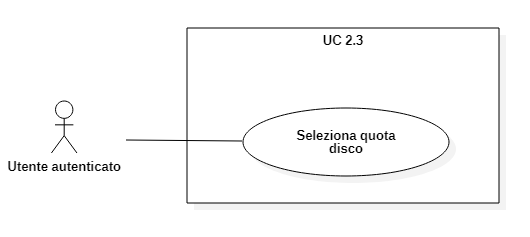
\includegraphics[scale = 0.7]{components/img/UC2_3.png}
    \caption{UC2.3 - Seleziona quota disco}
\end{figure}
\begin{itemize}
\item \textbf{Attore Primario:} Utente autenticato;
\item \textbf{Precondizione:} L'utente vuole cambiare la dimensione dei file che l'applicazione scaricherà dal server;
\item \textbf{Postcondizione:} L'utente ha deciso che file superiori al limite imposto non verranno scaricati;
\item \textbf{Scenario principale:}
    \begin{enumerate}
    \item L'utente ha poco spazio all'interno del computer;
    \item L'utente decide di inserire un filtro che limita l'applicazione da scaricare file troppo grandi.
    \end{enumerate}
\end{itemize}

\subsubsection{UC2.4 - Logout}
\begin{figure}[H]
    \centering
    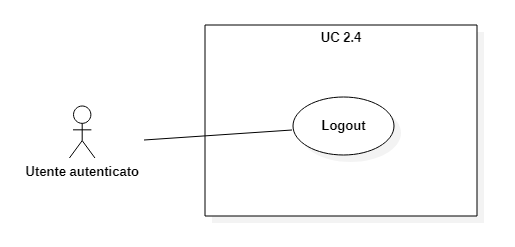
\includegraphics[scale = 0.7]{components/img/UC2_4.png}
    \caption{UC2.4 - Logout}
\end{figure}
\begin{itemize}
\item \textbf{Attore Primario:} Utente autenticato;
\item \textbf{Precondizione:} L'utente vuole effettuare il logout;
\item \textbf{Postcondizione:} L'utente ha effettuato il logout e non è più riconoscibile all'interno dell'applicazione;
\item \textbf{Scenario principale:}
    \begin{enumerate}
    \item L'utente vuole effettuare il logout;
    \item L'utente ha effettuato il logout;
    \item Tutti i file che l'utente in precedenza sincronizzava non vengono più sincronizzati con il server.
    \end{enumerate}
\end{itemize}
%Visualizza impostazioni

\subsection{UC3 - Sincronizzazione file da server a client}
\label{UC3}
\begin{figure}[H]
    \centering
    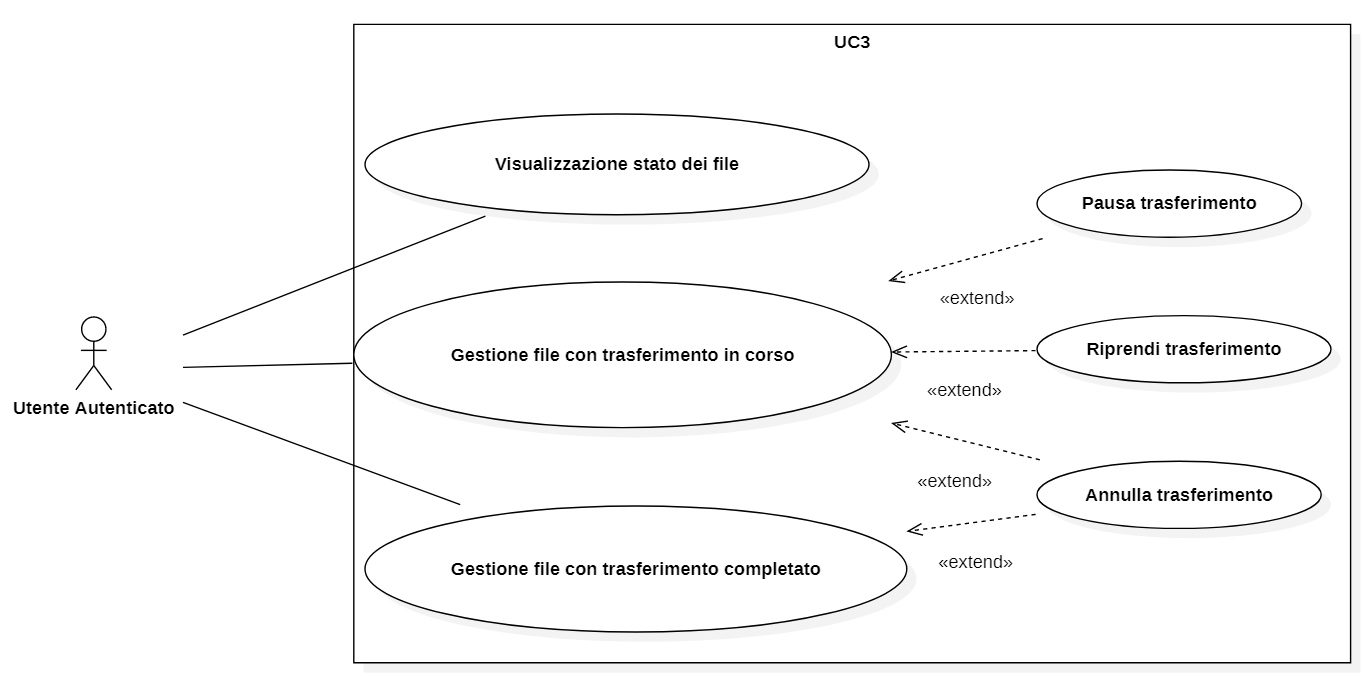
\includegraphics[scale = 0.5]{components/img/UC3.png}
    \caption{UC3 - Sincronizzazione file da server a client}
\end{figure}
\begin{itemize}
\item \textbf{Attore Primario:} Utente autenticato;
\item \textbf{Attore Secondario:} \glo{Zextras Drive};
\item \textbf{Precondizione:} L'utente ha necessità di sincronizzare uno o più file dal server verso il client;
\item \textbf{Postcondizione:} L'utente ha sincronizzato i file dal server al client;
\item \textbf{Scenario principale:}
    \begin{enumerate}
    \item L'utente vuole sincronizzare dei file dal server al client;
    \item Viene scelto l'insieme dei file che dovrà essere sincronizzato;
    \item La sincronizzazione delle modifiche viene attivata per l'insieme scelto.
    \end{enumerate}
\item \textbf{Estensioni:}
    \begin{itemize}
    \item Visualizza messaggio di errore di rete (UC7 \S{}\ref{UC7});
    \item Visualizza messaggio di errore spazio non disponibile in locale (UC10 \S{}\ref{UC10}).
\end{itemize}
\end{itemize}
%Visualizzazione dei trasferimenti

\subsection{UC4 - Seleziona quota disco}
\begin{figure}[H]
    \centering
    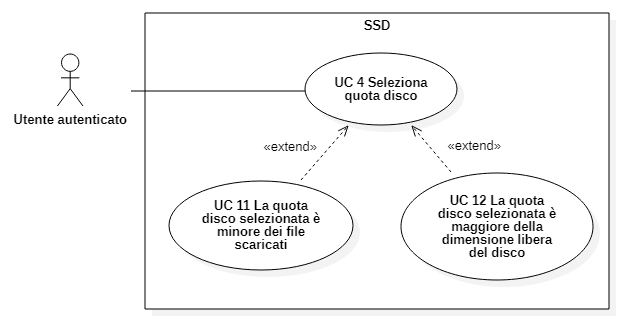
\includegraphics[scale = 0.6]{components/img/UC4.png}
    \caption{UC4 - Seleziona quota disco}
\end{figure}
\begin{itemize}
\item \textbf{Attore Primario:} Utente autenticato;
\item \textbf{Precondizione:} L'utente vuole cambiare la dimensione disco riservata, lato client, per le iterazioni con \glo{Zextras Drive};
\item \textbf{Postcondizione:} L'utente ha cambiato lo spazio disco riservato per l'applicativo;
\item \textbf{Scenario principale:}
    \begin{enumerate}
    \item L'utente necessita di cambiare lo spazio disco dedicato;
        \begin{itemize}
        \item L'utente ha poco spazio nel disco e vuole ridurre lo spazio dedicato per le iterazioni con \glo{Zextras Drive};
        \item L'utente ha abbastanza spazio disponibile da voler aumentare lo spazio disco dedicato per le iterazioni con \glo{Zextras Drive};
        \end{itemize}
    \item L'utente ha cambiato lo spazio disco dedicato;
    \end{enumerate}
\item \textbf{Estensioni:}
    \begin{itemize}
        \item La quota disco selezionata è minore dei file scaricati (UC11 \S{}\ref{UC11});
        \item La quota disco selezionata è maggiore della dimensione libera del disco (UC12 \S{}\ref{UC12})
    \end{itemize}
\end{itemize}%Visualizzazione messaggio di errore inserimento credenziali

\subsection{UC5 - Visualizzazione messaggio di errore di rete}
\label{UC5}
\begin{itemize}
\item \textbf{Attore Primario:} Utente autenticato;
\item \textbf{Precondizione:} Il \glo{sistema} prova a comunicare con \glo{Zextras Drive};
\item \textbf{Postcondizione:} L'utente viene informato che non è stato possibile completare la sincronizzazione;
\item \textbf{Scenario principale:}
    \begin{enumerate}
    \item L'utente ha selezionato i file da sincronizzare;
    \item L'applicazione prova a connettersi a \glo{Zextras Drive}, ma fallisce per assenza di rete.
    \end{enumerate}
\end{itemize}%Visualizzazione messaggio di errore di rete

\subsection{UC6 - Visualizza dettagli file}
\label{UC6}
\begin{figure}[H]
    \centering
    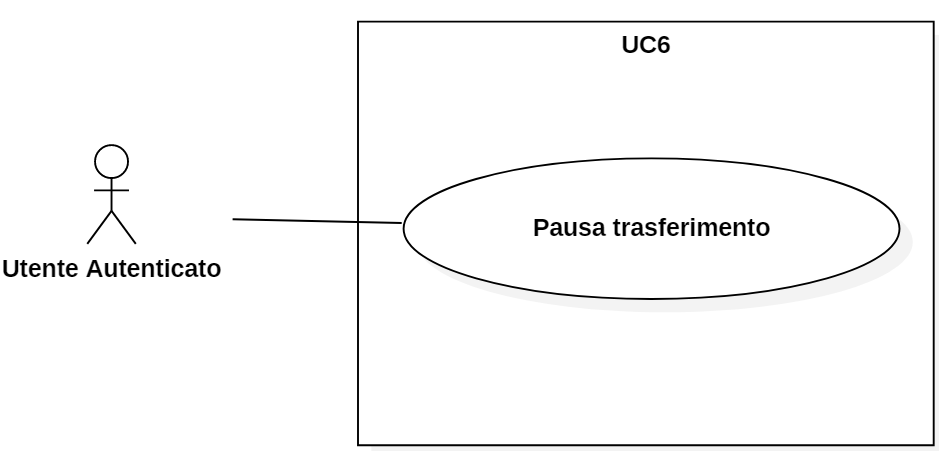
\includegraphics[scale = 0.6]{components/img/UC6.png}
    \caption{UC6 - Visualizza dettagli file}
\end{figure}
\begin{itemize}
\item \textbf{Attore Primario:} Utente autenticato;
\item \textbf{Precondizione:} L'utente ha selezionato la cartella root e sono presenti file al suo interno;
\item \textbf{Postcondizione:} L'utente ha informazioni riguardo al file;
\item \textbf{Scenario principale:} L'utente può visualizzare le informazioni riguardanti i file all'interno della cartella root selezionata.
\end{itemize}

\subsubsection{UC6.1 - Visualizza data creazione file}
\label{UC6.1}
\begin{itemize}
\item \textbf{Attore Primario:} Utente autenticato;
\item \textbf{Precondizione:} L'utente ha selezionato la cartella root e sono presenti file al suo interno;
\item \textbf{Postcondizione:} L'utente è informato sulla data di creazione del file;
\item \textbf{Scenario principale:} L'utente può visualizzare la data di creazione dei file.
\end{itemize}

\subsubsection{UC6.2 - Visualizza data ultima modifica file}
\label{UC6.2}
\begin{itemize}
\item \textbf{Attore Primario:} Utente autenticato;
\item \textbf{Precondizione:} L'utente ha selezionato la cartella root e sono presenti file al suo interno;
\item \textbf{Postcondizione:} L'utente è informato sulla data di ultima modifica del file;
\item \textbf{Scenario principale:} L'utente può visualizzare la data di ultima modifica dei file.
\end{itemize}

\subsubsection{UC6.3 - Visualizza grandezza file}
\label{UC6.3}
\begin{itemize}
\item \textbf{Attore Primario:} Utente autenticato;
\item \textbf{Precondizione:} L'utente ha selezionato la cartella root e sono presenti file al suo interno;
\item \textbf{Postcondizione:} L'utente è informato sulla grandezza del file;
\item \textbf{Scenario principale:} L'utente può visualizzare la grandezza dei file.
\end{itemize}

\subsubsection{UC6.4 - Visualizza stato dei file}
\label{UC6.4}
\begin{itemize}
\item \textbf{Attore Primario:} Utente autenticato;
\item \textbf{Precondizione:} L'utente ha effettuato dei trasferimenti da o verso il server;
\item \textbf{Postcondizione:} L'utente è informato sullo stato dei file sincronizzati e non;
\item \textbf{Scenario principale:} L'utente può visualizzare lo stato corrente dei file.
\end{itemize}
%Visualizzazione messaggio di errore file troppo grande

\subsection{UC7 - Riprendi trasferimento}
\begin{figure}[H]
    \centering
    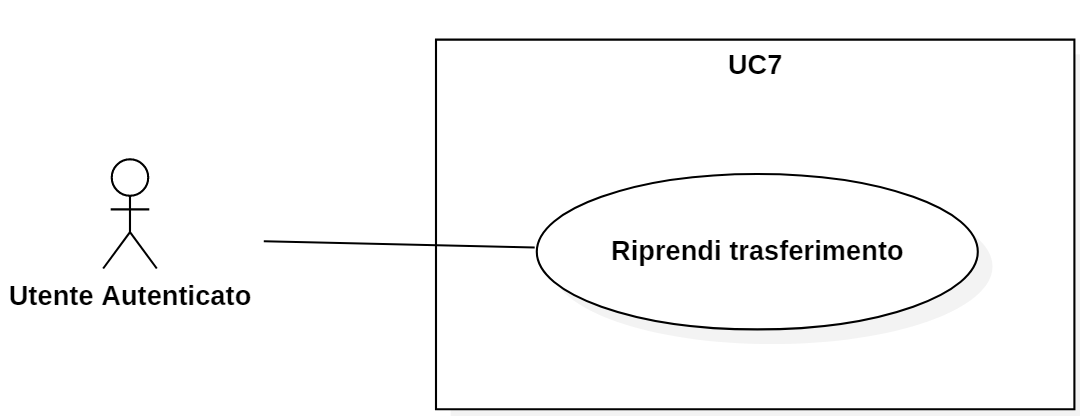
\includegraphics[scale = 0.4]{components/img/UC7.png}
    \caption{UC7 - Riprendi trasferimento}
\end{figure}
\begin{itemize}
\item \textbf{Attore Primario:} Utente autenticato;
\item \textbf{Precondizione:} L'utente ha a disposizione la possibilità di riprendere il trasferimento di un file messo precedentemente in pausa;
\item \textbf{Postcondizione:} Viene modificato lo stato del file da trasferimento in pausa a trasferimento in corso;
\item \textbf{Scenario principale:}
    \begin{enumerate}
    \item L'utente può riprendere il trasferimento di un file che si trova nello stato di trasferimento in pausa.
    \end{enumerate}
\end{itemize}

